\begin{figure}
\centering
%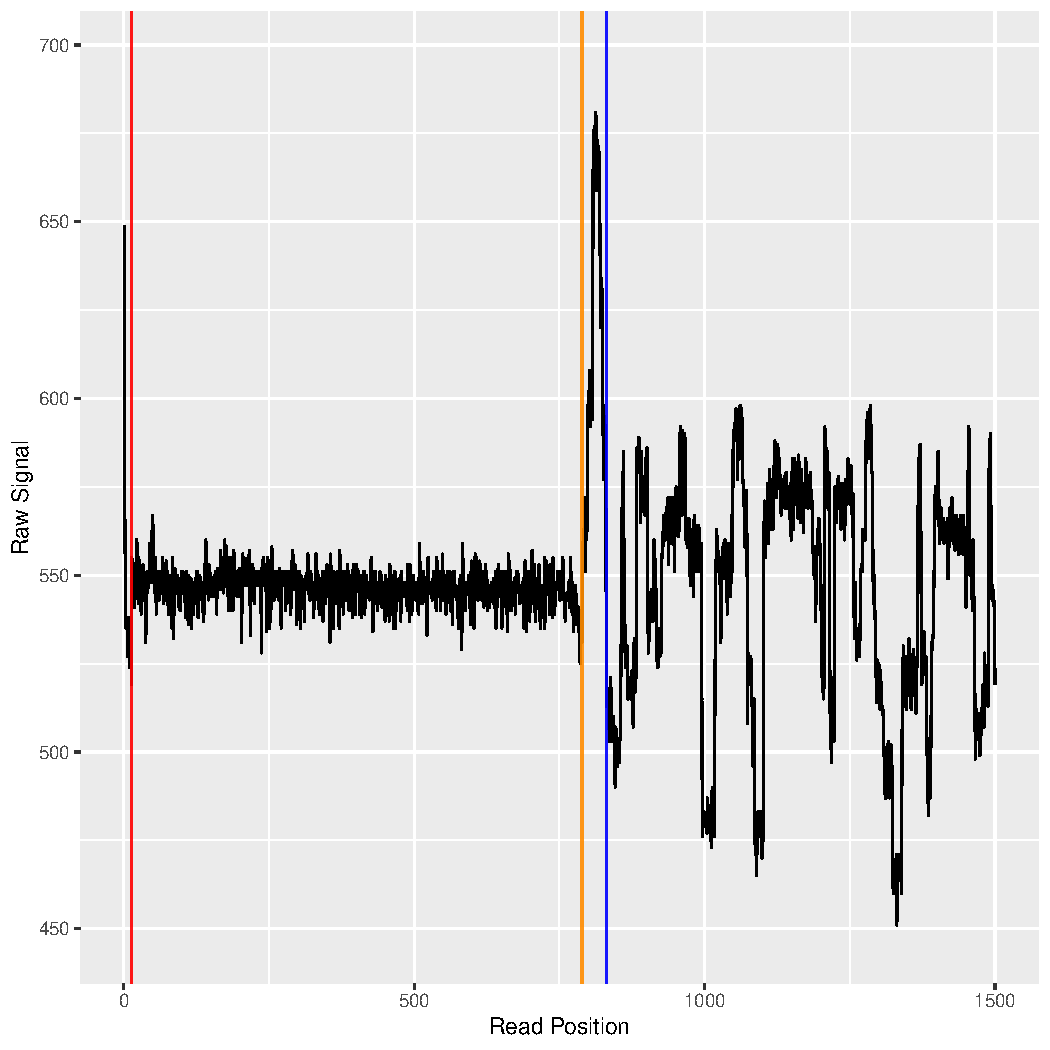
\includegraphics[scale=0.7]{plots/reads.e9f08690-171f-476f-9119-5330d0290126.raw.section.pdf}
% Created by tikzDevice version 0.12.3.1 on 2022-09-19 17:22:31
% !TEX encoding = UTF-8 Unicode
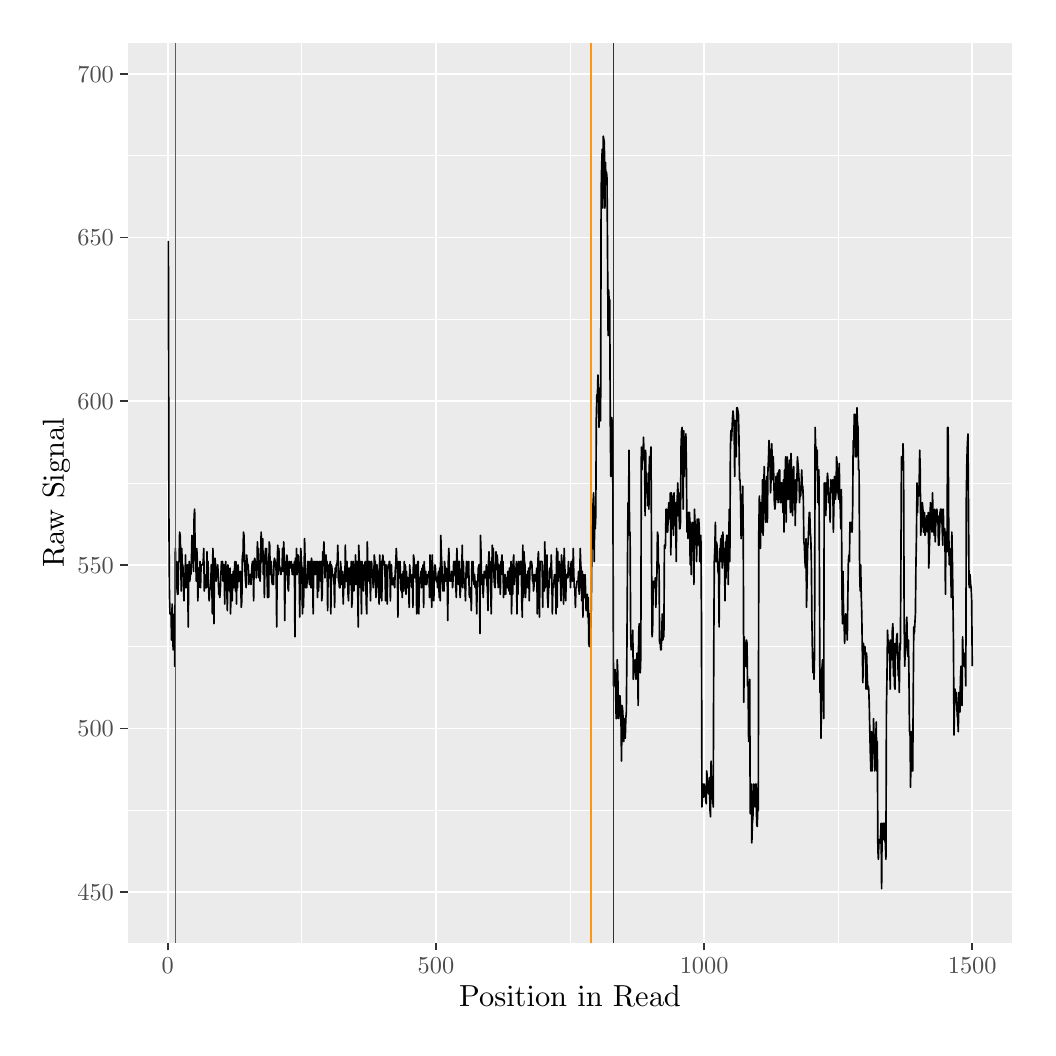
\begin{tikzpicture}[x=1pt,y=1pt]
\definecolor{fillColor}{RGB}{255,255,255}
\path[use as bounding box,fill=fillColor,fill opacity=0.00] (0,0) rectangle (361.35,361.35);
\begin{scope}
\path[clip] (  0.00,  0.00) rectangle (361.35,361.35);
\definecolor{drawColor}{RGB}{255,255,255}
\definecolor{fillColor}{RGB}{255,255,255}

\path[draw=drawColor,line width= 0.6pt,line join=round,line cap=round,fill=fillColor] (  0.00,  0.00) rectangle (361.35,361.35);
\end{scope}
\begin{scope}
\path[clip] ( 36.11, 30.69) rectangle (355.85,355.85);
\definecolor{fillColor}{gray}{0.92}

\path[fill=fillColor] ( 36.11, 30.69) rectangle (355.85,355.85);
\definecolor{drawColor}{RGB}{255,255,255}

\path[draw=drawColor,line width= 0.3pt,line join=round] ( 36.11, 78.57) --
	(355.85, 78.57);

\path[draw=drawColor,line width= 0.3pt,line join=round] ( 36.11,137.69) --
	(355.85,137.69);

\path[draw=drawColor,line width= 0.3pt,line join=round] ( 36.11,196.82) --
	(355.85,196.82);

\path[draw=drawColor,line width= 0.3pt,line join=round] ( 36.11,255.94) --
	(355.85,255.94);

\path[draw=drawColor,line width= 0.3pt,line join=round] ( 36.11,315.06) --
	(355.85,315.06);

\path[draw=drawColor,line width= 0.3pt,line join=round] ( 99.09, 30.69) --
	( 99.09,355.85);

\path[draw=drawColor,line width= 0.3pt,line join=round] (195.98, 30.69) --
	(195.98,355.85);

\path[draw=drawColor,line width= 0.3pt,line join=round] (292.87, 30.69) --
	(292.87,355.85);

\path[draw=drawColor,line width= 0.6pt,line join=round] ( 36.11, 49.01) --
	(355.85, 49.01);

\path[draw=drawColor,line width= 0.6pt,line join=round] ( 36.11,108.13) --
	(355.85,108.13);

\path[draw=drawColor,line width= 0.6pt,line join=round] ( 36.11,167.25) --
	(355.85,167.25);

\path[draw=drawColor,line width= 0.6pt,line join=round] ( 36.11,226.38) --
	(355.85,226.38);

\path[draw=drawColor,line width= 0.6pt,line join=round] ( 36.11,285.50) --
	(355.85,285.50);

\path[draw=drawColor,line width= 0.6pt,line join=round] ( 36.11,344.62) --
	(355.85,344.62);

\path[draw=drawColor,line width= 0.6pt,line join=round] ( 50.64, 30.69) --
	( 50.64,355.85);

\path[draw=drawColor,line width= 0.6pt,line join=round] (147.54, 30.69) --
	(147.54,355.85);

\path[draw=drawColor,line width= 0.6pt,line join=round] (244.43, 30.69) --
	(244.43,355.85);

\path[draw=drawColor,line width= 0.6pt,line join=round] (341.32, 30.69) --
	(341.32,355.85);
\definecolor{drawColor}{RGB}{0,0,0}

\path[draw=drawColor,line width= 0.6pt,line join=round] ( 50.84,284.31) --
	( 51.03,184.99) --
	( 51.23,156.61) --
	( 51.42,149.52) --
	( 51.61,149.52) --
	( 51.81,149.52) --
	( 52.00,140.06) --
	( 52.20,153.07) --
	( 52.39,142.42) --
	( 52.58,136.51) --
	( 52.78,144.79) --
	( 52.97,149.52) --
	( 53.16,130.60) --
	( 53.36,173.17) --
	( 53.55,164.89) --
	( 53.75,168.44) --
	( 53.94,158.98) --
	( 54.13,156.61) --
	( 54.33,156.61) --
	( 54.52,168.44) --
	( 54.71,168.44) --
	( 54.91,179.08) --
	( 55.10,177.90) --
	( 55.30,170.80) --
	( 55.49,157.80) --
	( 55.68,173.17) --
	( 55.88,166.07) --
	( 56.07,167.25) --
	( 56.26,162.53) --
	( 56.46,154.25) --
	( 56.65,163.71) --
	( 56.85,161.34) --
	( 57.04,170.80) --
	( 57.23,158.98) --
	( 57.43,160.16) --
	( 57.62,162.53) --
	( 57.81,167.25) --
	( 58.01,144.79) --
	( 58.20,164.89) --
	( 58.40,168.44) --
	( 58.59,161.34) --
	( 58.78,163.71) --
	( 58.98,163.71) --
	( 59.17,168.44) --
	( 59.36,177.90) --
	( 59.56,175.53) --
	( 59.75,170.80) --
	( 59.95,164.89) --
	( 60.14,184.99) --
	( 60.33,187.36) --
	( 60.53,170.80) --
	( 60.72,170.80) --
	( 60.92,161.34) --
	( 61.11,173.17) --
	( 61.30,168.44) --
	( 61.50,154.25) --
	( 61.69,166.07) --
	( 61.88,158.98) --
	( 62.08,162.53) --
	( 62.27,168.44) --
	( 62.47,158.98) --
	( 62.66,167.25) --
	( 62.85,167.25) --
	( 63.05,167.25) --
	( 63.24,167.25) --
	( 63.43,168.44) --
	( 63.63,173.17) --
	( 63.82,157.80) --
	( 64.02,163.71) --
	( 64.21,158.98) --
	( 64.40,158.98) --
	( 64.60,158.98) --
	( 64.79,171.98) --
	( 64.98,163.71) --
	( 65.18,168.44) --
	( 65.37,158.98) --
	( 65.57,154.25) --
	( 65.76,157.80) --
	( 65.95,158.98) --
	( 66.15,158.98) --
	( 66.34,167.25) --
	( 66.53,161.34) --
	( 66.73,149.52) --
	( 66.92,173.17) --
	( 67.12,166.07) --
	( 67.31,145.97) --
	( 67.50,168.44) --
	( 67.70,169.62) --
	( 67.89,167.25) --
	( 68.09,161.34) --
	( 68.28,163.71) --
	( 68.47,164.89) --
	( 68.67,167.25) --
	( 68.86,163.71) --
	( 69.05,156.61) --
	( 69.25,156.61) --
	( 69.44,155.43) --
	( 69.64,158.98) --
	( 69.83,163.71) --
	( 70.02,168.44) --
	( 70.22,166.07) --
	( 70.41,168.44) --
	( 70.60,161.34) --
	( 70.80,167.25) --
	( 70.99,167.25) --
	( 71.19,153.07) --
	( 71.38,163.71) --
	( 71.57,168.44) --
	( 71.77,163.71) --
	( 71.96,158.98) --
	( 72.15,150.70) --
	( 72.35,167.25) --
	( 72.54,164.89) --
	( 72.74,164.89) --
	( 72.93,157.80) --
	( 73.12,166.07) --
	( 73.32,149.52) --
	( 73.51,163.71) --
	( 73.70,163.71) --
	( 73.90,154.25) --
	( 74.09,162.53) --
	( 74.29,164.89) --
	( 74.48,158.98) --
	( 74.67,163.71) --
	( 74.87,168.44) --
	( 75.06,157.80) --
	( 75.25,168.44) --
	( 75.45,153.07) --
	( 75.64,166.07) --
	( 75.84,158.98) --
	( 76.03,167.25) --
	( 76.22,163.71) --
	( 76.42,161.34) --
	( 76.61,163.71) --
	( 76.81,164.89) --
	( 77.00,160.16) --
	( 77.19,151.88) --
	( 77.39,154.25) --
	( 77.58,170.80) --
	( 77.77,168.44) --
	( 77.97,179.08) --
	( 78.16,177.90) --
	( 78.36,169.62) --
	( 78.55,164.89) --
	( 78.74,161.34) --
	( 78.94,158.98) --
	( 79.13,170.80) --
	( 79.32,168.44) --
	( 79.52,167.25) --
	( 79.71,167.25) --
	( 79.91,160.16) --
	( 80.10,163.71) --
	( 80.29,163.71) --
	( 80.49,163.71) --
	( 80.68,160.16) --
	( 80.87,163.71) --
	( 81.07,167.25) --
	( 81.26,168.44) --
	( 81.46,168.44) --
	( 81.65,154.25) --
	( 81.84,168.44) --
	( 82.04,169.62) --
	( 82.23,168.44) --
	( 82.42,168.44) --
	( 82.62,162.53) --
	( 82.81,163.71) --
	( 83.01,175.53) --
	( 83.20,168.44) --
	( 83.39,173.17) --
	( 83.59,162.53) --
	( 83.78,163.71) --
	( 83.98,161.34) --
	( 84.17,166.07) --
	( 84.36,179.08) --
	( 84.56,168.44) --
	( 84.75,170.80) --
	( 84.94,176.71) --
	( 85.14,163.71) --
	( 85.33,170.80) --
	( 85.53,155.43) --
	( 85.72,167.25) --
	( 85.91,173.17) --
	( 86.11,168.44) --
	( 86.30,173.17) --
	( 86.49,163.71) --
	( 86.69,155.43) --
	( 86.88,168.44) --
	( 87.08,155.43) --
	( 87.27,175.53) --
	( 87.46,174.35) --
	( 87.66,163.71) --
	( 87.85,168.44) --
	( 88.04,168.44) --
	( 88.24,161.34) --
	( 88.43,160.16) --
	( 88.63,161.34) --
	( 88.82,160.16) --
	( 89.01,168.44) --
	( 89.21,169.62) --
	( 89.40,168.44) --
	( 89.59,167.25) --
	( 89.79,164.89) --
	( 89.98,144.79) --
	( 90.18,168.44) --
	( 90.37,174.35) --
	( 90.56,163.71) --
	( 90.76,173.17) --
	( 90.95,167.25) --
	( 91.15,166.07) --
	( 91.34,164.89) --
	( 91.53,163.71) --
	( 91.73,166.07) --
	( 91.92,166.07) --
	( 92.11,173.17) --
	( 92.31,164.89) --
	( 92.50,175.53) --
	( 92.70,170.80) --
	( 92.89,147.15) --
	( 93.08,164.89) --
	( 93.28,168.44) --
	( 93.47,163.71) --
	( 93.66,170.80) --
	( 93.86,168.44) --
	( 94.05,158.98) --
	( 94.25,157.80) --
	( 94.44,164.89) --
	( 94.63,168.44) --
	( 94.83,166.07) --
	( 95.02,167.25) --
	( 95.21,168.44) --
	( 95.41,167.25) --
	( 95.60,163.71) --
	( 95.80,167.25) --
	( 95.99,163.71) --
	( 96.18,164.89) --
	( 96.38,168.44) --
	( 96.57,141.24) --
	( 96.76,169.62) --
	( 96.96,163.71) --
	( 97.15,173.17) --
	( 97.35,163.71) --
	( 97.54,170.80) --
	( 97.73,170.80) --
	( 97.93,166.07) --
	( 98.12,163.71) --
	( 98.31,148.34) --
	( 98.51,167.25) --
	( 98.70,173.17) --
	( 98.90,168.44) --
	( 99.09,166.07) --
	( 99.28,149.52) --
	( 99.48,166.07) --
	( 99.67,151.88) --
	( 99.87,163.71) --
	(100.06,176.71) --
	(100.25,168.44) --
	(100.45,158.98) --
	(100.64,163.71) --
	(100.83,158.98) --
	(101.03,162.53) --
	(101.22,168.44) --
	(101.42,168.44) --
	(101.61,164.89) --
	(101.80,160.16) --
	(102.00,168.44) --
	(102.19,160.16) --
	(102.38,158.98) --
	(102.58,169.62) --
	(102.77,167.25) --
	(102.97,163.71) --
	(103.16,149.52) --
	(103.35,168.44) --
	(103.55,163.71) --
	(103.74,168.44) --
	(103.93,163.71) --
	(104.13,168.44) --
	(104.32,164.89) --
	(104.52,168.44) --
	(104.71,155.43) --
	(104.90,168.44) --
	(105.10,157.80) --
	(105.29,162.53) --
	(105.48,168.44) --
	(105.68,168.44) --
	(105.87,161.34) --
	(106.07,168.44) --
	(106.26,154.25) --
	(106.45,156.61) --
	(106.65,171.98) --
	(106.84,168.44) --
	(107.04,175.53) --
	(107.23,168.44) --
	(107.42,162.53) --
	(107.62,168.44) --
	(107.81,170.80) --
	(108.00,164.89) --
	(108.20,168.44) --
	(108.39,150.70) --
	(108.59,167.25) --
	(108.78,163.71) --
	(108.97,162.53) --
	(109.17,167.25) --
	(109.36,168.44) --
	(109.55,149.52) --
	(109.75,167.25) --
	(109.94,166.07) --
	(110.14,163.71) --
	(110.33,163.71) --
	(110.52,162.53) --
	(110.72,160.16) --
	(110.91,151.88) --
	(111.10,166.07) --
	(111.30,162.53) --
	(111.49,167.25) --
	(111.69,167.25) --
	(111.88,168.44) --
	(112.07,174.35) --
	(112.27,161.34) --
	(112.46,161.34) --
	(112.65,158.98) --
	(112.85,158.98) --
	(113.04,168.44) --
	(113.24,166.07) --
	(113.43,160.16) --
	(113.62,160.16) --
	(113.82,164.89) --
	(114.01,153.07) --
	(114.20,160.16) --
	(114.40,163.71) --
	(114.59,158.98) --
	(114.79,174.35) --
	(114.98,161.34) --
	(115.17,161.34) --
	(115.37,168.44) --
	(115.56,164.89) --
	(115.76,156.61) --
	(115.95,154.25) --
	(116.14,166.07) --
	(116.34,166.07) --
	(116.53,160.16) --
	(116.72,162.53) --
	(116.92,168.44) --
	(117.11,151.88) --
	(117.31,155.43) --
	(117.50,168.44) --
	(117.69,168.44) --
	(117.89,157.80) --
	(118.08,167.25) --
	(118.27,160.16) --
	(118.47,170.80) --
	(118.66,160.16) --
	(118.86,168.44) --
	(119.05,168.44) --
	(119.24,160.16) --
	(119.44,144.79) --
	(119.63,174.35) --
	(119.82,168.44) --
	(120.02,167.25) --
	(120.21,158.98) --
	(120.41,168.44) --
	(120.60,149.52) --
	(120.79,168.44) --
	(120.99,166.07) --
	(121.18,161.34) --
	(121.37,157.80) --
	(121.57,167.25) --
	(121.76,167.25) --
	(121.96,168.44) --
	(122.15,163.71) --
	(122.34,153.07) --
	(122.54,149.52) --
	(122.73,175.53) --
	(122.93,164.89) --
	(123.12,162.53) --
	(123.31,161.34) --
	(123.51,168.44) --
	(123.70,161.34) --
	(123.89,154.25) --
	(124.09,168.44) --
	(124.28,168.44) --
	(124.48,163.71) --
	(124.67,163.71) --
	(124.86,158.98) --
	(125.06,161.34) --
	(125.25,170.80) --
	(125.44,168.44) --
	(125.64,168.44) --
	(125.83,155.43) --
	(126.03,158.98) --
	(126.22,167.25) --
	(126.41,163.71) --
	(126.61,164.89) --
	(126.80,158.98) --
	(126.99,153.07) --
	(127.19,170.80) --
	(127.38,162.53) --
	(127.58,155.43) --
	(127.77,168.44) --
	(127.96,154.25) --
	(128.16,168.44) --
	(128.35,170.80) --
	(128.54,167.25) --
	(128.74,168.44) --
	(128.93,168.44) --
	(129.13,163.71) --
	(129.32,154.25) --
	(129.51,167.25) --
	(129.71,163.71) --
	(129.90,153.07) --
	(130.10,166.07) --
	(130.29,167.25) --
	(130.48,166.07) --
	(130.68,168.44) --
	(130.87,168.44) --
	(131.06,154.25) --
	(131.26,166.07) --
	(131.45,167.25) --
	(131.65,160.16) --
	(131.84,160.16) --
	(132.03,160.16) --
	(132.23,162.53) --
	(132.42,160.16) --
	(132.61,158.98) --
	(132.81,164.89) --
	(133.00,167.25) --
	(133.20,173.17) --
	(133.39,168.44) --
	(133.58,166.07) --
	(133.78,148.34) --
	(133.97,168.44) --
	(134.16,163.71) --
	(134.36,162.53) --
	(134.55,168.44) --
	(134.75,162.53) --
	(134.94,157.80) --
	(135.13,163.71) --
	(135.33,155.43) --
	(135.52,162.53) --
	(135.71,164.89) --
	(135.91,157.80) --
	(136.10,168.44) --
	(136.30,163.71) --
	(136.49,167.25) --
	(136.68,156.61) --
	(136.88,164.89) --
	(137.07,160.16) --
	(137.26,158.98) --
	(137.46,162.53) --
	(137.65,160.16) --
	(137.85,151.88) --
	(138.04,167.25) --
	(138.23,163.71) --
	(138.43,163.71) --
	(138.62,162.53) --
	(138.82,158.98) --
	(139.01,163.71) --
	(139.20,151.88) --
	(139.40,170.80) --
	(139.59,169.62) --
	(139.78,166.07) --
	(139.98,162.53) --
	(140.17,166.07) --
	(140.37,167.25) --
	(140.56,149.52) --
	(140.75,163.71) --
	(140.95,168.44) --
	(141.14,168.44) --
	(141.33,149.52) --
	(141.53,160.16) --
	(141.72,162.53) --
	(141.92,161.34) --
	(142.11,164.89) --
	(142.30,158.98) --
	(142.50,166.07) --
	(142.69,162.53) --
	(142.88,167.25) --
	(143.08,151.88) --
	(143.27,168.44) --
	(143.47,163.71) --
	(143.66,160.16) --
	(143.85,164.89) --
	(144.05,160.16) --
	(144.24,160.16) --
	(144.43,163.71) --
	(144.63,163.71) --
	(144.82,163.71) --
	(145.02,164.89) --
	(145.21,155.43) --
	(145.40,170.80) --
	(145.60,161.34) --
	(145.79,162.53) --
	(145.99,151.88) --
	(146.18,170.80) --
	(146.37,163.71) --
	(146.57,160.16) --
	(146.76,154.25) --
	(146.95,163.71) --
	(147.15,167.25) --
	(147.34,166.07) --
	(147.54,162.53) --
	(147.73,161.34) --
	(147.92,162.53) --
	(148.12,158.98) --
	(148.31,163.71) --
	(148.50,164.89) --
	(148.70,155.43) --
	(148.89,166.07) --
	(149.09,154.25) --
	(149.28,177.90) --
	(149.47,170.80) --
	(149.67,167.25) --
	(149.86,161.34) --
	(150.05,157.80) --
	(150.25,162.53) --
	(150.44,157.80) --
	(150.64,168.44) --
	(150.83,166.07) --
	(151.02,161.34) --
	(151.22,166.07) --
	(151.41,164.89) --
	(151.60,162.53) --
	(151.80,147.15) --
	(151.99,168.44) --
	(152.19,173.17) --
	(152.38,163.71) --
	(152.57,161.34) --
	(152.77,163.71) --
	(152.96,161.34) --
	(153.15,164.89) --
	(153.35,163.71) --
	(153.54,158.98) --
	(153.74,162.53) --
	(153.93,168.44) --
	(154.12,163.71) --
	(154.32,168.44) --
	(154.51,168.44) --
	(154.71,158.98) --
	(154.90,155.43) --
	(155.09,173.17) --
	(155.29,166.07) --
	(155.48,163.71) --
	(155.67,160.16) --
	(155.87,168.44) --
	(156.06,168.44) --
	(156.26,155.43) --
	(156.45,158.98) --
	(156.64,163.71) --
	(156.84,163.71) --
	(157.03,174.35) --
	(157.22,158.98) --
	(157.42,168.44) --
	(157.61,162.53) --
	(157.81,161.34) --
	(158.00,160.16) --
	(158.19,154.25) --
	(158.39,163.71) --
	(158.58,168.44) --
	(158.77,168.44) --
	(158.97,163.71) --
	(159.16,162.53) --
	(159.36,168.44) --
	(159.55,156.61) --
	(159.74,155.43) --
	(159.94,158.98) --
	(160.13,156.61) --
	(160.32,150.70) --
	(160.52,168.44) --
	(160.71,167.25) --
	(160.91,168.44) --
	(161.10,163.71) --
	(161.29,160.16) --
	(161.49,163.71) --
	(161.68,158.98) --
	(161.88,161.34) --
	(162.07,158.98) --
	(162.26,149.52) --
	(162.46,161.34) --
	(162.65,161.34) --
	(162.84,166.07) --
	(163.04,167.25) --
	(163.23,167.25) --
	(163.43,142.42) --
	(163.62,177.90) --
	(163.81,171.98) --
	(164.01,160.16) --
	(164.20,163.71) --
	(164.39,163.71) --
	(164.59,155.43) --
	(164.78,160.16) --
	(164.98,164.89) --
	(165.17,164.89) --
	(165.36,162.53) --
	(165.56,162.53) --
	(165.75,167.25) --
	(165.94,160.16) --
	(166.14,158.98) --
	(166.33,150.70) --
	(166.53,168.44) --
	(166.72,171.98) --
	(166.91,162.53) --
	(167.11,168.44) --
	(167.30,161.34) --
	(167.49,149.52) --
	(167.69,162.53) --
	(167.88,174.35) --
	(168.08,166.07) --
	(168.27,173.17) --
	(168.46,163.71) --
	(168.66,160.16) --
	(168.85,158.98) --
	(169.05,162.53) --
	(169.24,171.98) --
	(169.43,168.44) --
	(169.63,170.80) --
	(169.82,168.44) --
	(170.01,158.98) --
	(170.21,167.25) --
	(170.40,163.71) --
	(170.60,163.71) --
	(170.79,156.61) --
	(170.98,168.44) --
	(171.18,166.07) --
	(171.37,170.80) --
	(171.56,163.71) --
	(171.76,168.44) --
	(171.95,155.43) --
	(172.15,158.98) --
	(172.34,156.61) --
	(172.53,163.71) --
	(172.73,156.61) --
	(172.92,162.53) --
	(173.11,162.53) --
	(173.31,158.98) --
	(173.50,164.89) --
	(173.70,161.34) --
	(173.89,157.80) --
	(174.08,166.07) --
	(174.28,156.61) --
	(174.47,163.71) --
	(174.66,168.44) --
	(174.86,149.52) --
	(175.05,167.25) --
	(175.25,156.61) --
	(175.44,168.44) --
	(175.63,170.80) --
	(175.83,160.16) --
	(176.02,163.71) --
	(176.21,166.07) --
	(176.41,163.71) --
	(176.60,168.44) --
	(176.80,149.52) --
	(176.99,166.07) --
	(177.18,156.61) --
	(177.38,168.44) --
	(177.57,164.89) --
	(177.77,163.71) --
	(177.96,168.44) --
	(178.15,168.44) --
	(178.35,168.44) --
	(178.54,154.25) --
	(178.73,148.34) --
	(178.93,174.35) --
	(179.12,155.43) --
	(179.32,171.98) --
	(179.51,168.44) --
	(179.70,167.25) --
	(179.90,155.43) --
	(180.09,161.34) --
	(180.28,163.71) --
	(180.48,158.98) --
	(180.67,164.89) --
	(180.87,163.71) --
	(181.06,166.07) --
	(181.25,154.25) --
	(181.45,164.89) --
	(181.64,168.44) --
	(181.83,168.44) --
	(182.03,168.44) --
	(182.22,167.25) --
	(182.42,161.34) --
	(182.61,163.71) --
	(182.80,157.80) --
	(183.00,160.16) --
	(183.19,163.71) --
	(183.38,161.34) --
	(183.58,162.53) --
	(183.77,163.71) --
	(183.97,166.07) --
	(184.16,149.52) --
	(184.35,168.44) --
	(184.55,171.98) --
	(184.74,158.98) --
	(184.94,148.34) --
	(185.13,168.44) --
	(185.32,168.44) --
	(185.52,168.44) --
	(185.71,168.44) --
	(185.90,168.44) --
	(186.10,151.88) --
	(186.29,164.89) --
	(186.49,161.34) --
	(186.68,157.80) --
	(186.87,175.53) --
	(187.07,158.98) --
	(187.26,162.53) --
	(187.45,167.25) --
	(187.65,170.80) --
	(187.84,155.43) --
	(188.04,151.88) --
	(188.23,158.98) --
	(188.42,158.98) --
	(188.62,166.07) --
	(188.81,163.71) --
	(189.00,162.53) --
	(189.20,170.80) --
	(189.39,163.71) --
	(189.59,149.52) --
	(189.78,160.16) --
	(189.97,158.98) --
	(190.17,161.34) --
	(190.36,163.71) --
	(190.55,163.71) --
	(190.75,161.34) --
	(190.94,149.52) --
	(191.14,173.17) --
	(191.33,151.88) --
	(191.52,171.98) --
	(191.72,161.34) --
	(191.91,164.89) --
	(192.10,168.44) --
	(192.30,164.89) --
	(192.49,163.71) --
	(192.69,154.25) --
	(192.88,170.80) --
	(193.07,168.44) --
	(193.27,164.89) --
	(193.46,158.98) --
	(193.66,153.07) --
	(193.85,173.17) --
	(194.04,167.25) --
	(194.24,163.71) --
	(194.43,154.25) --
	(194.62,163.71) --
	(194.82,163.71) --
	(195.01,163.71) --
	(195.21,162.53) --
	(195.40,168.44) --
	(195.59,163.71) --
	(195.79,166.07) --
	(195.98,163.71) --
	(196.17,158.98) --
	(196.37,168.44) --
	(196.56,168.44) --
	(196.76,166.07) --
	(196.95,161.34) --
	(197.14,173.17) --
	(197.34,163.71) --
	(197.53,158.98) --
	(197.72,158.98) --
	(197.92,151.88) --
	(198.11,158.98) --
	(198.31,158.98) --
	(198.50,161.34) --
	(198.69,161.34) --
	(198.89,161.34) --
	(199.08,164.89) --
	(199.27,156.61) --
	(199.47,158.98) --
	(199.66,173.17) --
	(199.86,167.25) --
	(200.05,164.89) --
	(200.24,154.25) --
	(200.44,164.89) --
	(200.63,148.34) --
	(200.83,163.71) --
	(201.02,158.98) --
	(201.21,155.43) --
	(201.41,163.71) --
	(201.60,157.80) --
	(201.79,150.70) --
	(201.99,155.43) --
	(202.18,156.61) --
	(202.38,148.34) --
	(202.57,155.43) --
	(202.76,138.88) --
	(202.96,137.69) --
	(203.15,149.52) --
	(203.34,149.52) --
	(203.54,144.79) --
	(203.73,158.98) --
	(203.93,181.44) --
	(204.12,173.17) --
	(204.31,189.72) --
	(204.51,193.27) --
	(204.70,168.44) --
	(204.89,184.99) --
	(205.09,180.26) --
	(205.28,184.99) --
	(205.48,220.46) --
	(205.67,228.74) --
	(205.86,227.56) --
	(206.06,235.83) --
	(206.25,228.74) --
	(206.44,216.92) --
	(206.64,231.11) --
	(206.83,231.11) --
	(207.03,219.28) --
	(207.22,302.05) --
	(207.41,311.51) --
	(207.61,317.42) --
	(207.80,296.14) --
	(208.00,322.15) --
	(208.19,320.97) --
	(208.38,319.79) --
	(208.58,296.14) --
	(208.77,312.69) --
	(208.96,306.78) --
	(209.16,309.14) --
	(209.35,306.78) --
	(209.55,277.22) --
	(209.74,250.02) --
	(209.93,266.58) --
	(210.13,261.85) --
	(210.32,263.03) --
	(210.51,220.46) --
	(210.71,199.18) --
	(210.90,219.28) --
	(211.10,220.46) --
	(211.29,212.19) --
	(211.48,193.27) --
	(211.68,123.51) --
	(211.87,128.24) --
	(212.06,123.51) --
	(212.26,129.42) --
	(212.45,122.32) --
	(212.65,111.68) --
	(212.84,111.68) --
	(213.03,132.96) --
	(213.23,128.24) --
	(213.42,117.59) --
	(213.61,111.68) --
	(213.81,115.23) --
	(214.00,119.96) --
	(214.20,116.41) --
	(214.39,111.68) --
	(214.58, 96.31) --
	(214.78,116.41) --
	(214.97,115.23) --
	(215.16,111.68) --
	(215.36,103.40) --
	(215.55,111.68) --
	(215.75,105.77) --
	(215.94,104.59) --
	(216.13,111.68) --
	(216.33,114.05) --
	(216.52,135.33) --
	(216.72,164.89) --
	(216.91,189.72) --
	(217.10,183.81) --
	(217.30,208.64) --
	(217.49,177.90) --
	(217.68,179.08) --
	(217.88,142.42) --
	(218.07,136.51) --
	(218.27,141.24) --
	(218.46,138.88) --
	(218.65,143.61) --
	(218.85,125.87) --
	(219.04,129.42) --
	(219.23,130.60) --
	(219.43,132.96) --
	(219.62,130.60) --
	(219.82,125.87) --
	(220.01,131.78) --
	(220.20,135.33) --
	(220.40,135.33) --
	(220.59,116.41) --
	(220.78,142.42) --
	(220.98,145.97) --
	(221.17,135.33) --
	(221.37,128.24) --
	(221.56,134.15) --
	(221.75,209.82) --
	(221.95,201.54) --
	(222.14,206.27) --
	(222.33,205.09) --
	(222.53,213.37) --
	(222.72,206.27) --
	(222.92,205.09) --
	(223.11,184.99) --
	(223.30,208.64) --
	(223.50,193.27) --
	(223.69,196.82) --
	(223.89,195.63) --
	(224.08,188.54) --
	(224.27,200.36) --
	(224.47,187.36) --
	(224.66,206.27) --
	(224.85,199.18) --
	(225.05,206.27) --
	(225.24,209.82) --
	(225.44,168.44) --
	(225.63,141.24) --
	(225.82,143.61) --
	(226.02,160.16) --
	(226.21,161.34) --
	(226.40,158.98) --
	(226.60,160.16) --
	(226.79,162.53) --
	(226.99,151.88) --
	(227.18,158.98) --
	(227.37,163.71) --
	(227.57,179.08) --
	(227.76,177.90) --
	(227.95,166.07) --
	(228.15,167.25) --
	(228.34,138.88) --
	(228.54,140.06) --
	(228.73,136.51) --
	(228.92,136.51) --
	(229.12,142.42) --
	(229.31,149.52) --
	(229.50,140.06) --
	(229.70,141.24) --
	(229.89,141.24) --
	(230.09,174.35) --
	(230.28,173.17) --
	(230.47,174.35) --
	(230.67,187.36) --
	(230.86,187.36) --
	(231.05,181.44) --
	(231.25,179.08) --
	(231.44,183.81) --
	(231.64,189.72) --
	(231.83,184.99) --
	(232.02,183.81) --
	(232.22,193.27) --
	(232.41,170.80) --
	(232.61,193.27) --
	(232.80,180.26) --
	(232.99,189.72) --
	(233.19,192.09) --
	(233.38,177.90) --
	(233.57,193.27) --
	(233.77,181.44) --
	(233.96,189.72) --
	(234.16,186.17) --
	(234.35,168.44) --
	(234.54,187.36) --
	(234.74,192.09) --
	(234.93,196.82) --
	(235.12,184.99) --
	(235.32,193.27) --
	(235.51,180.26) --
	(235.71,180.26) --
	(235.90,182.63) --
	(236.09,209.82) --
	(236.29,215.73) --
	(236.48,216.92) --
	(236.67,206.27) --
	(236.87,187.36) --
	(237.06,215.73) --
	(237.26,199.18) --
	(237.45,208.64) --
	(237.64,206.27) --
	(237.84,214.55) --
	(238.03,202.73) --
	(238.22,179.08) --
	(238.42,183.81) --
	(238.61,176.71) --
	(238.81,186.17) --
	(239.00,186.17) --
	(239.19,186.17) --
	(239.39,167.25) --
	(239.58,182.63) --
	(239.78,163.71) --
	(239.97,179.08) --
	(240.16,174.35) --
	(240.36,182.63) --
	(240.55,179.08) --
	(240.74,160.16) --
	(240.94,187.36) --
	(241.13,182.63) --
	(241.33,180.26) --
	(241.52,180.26) --
	(241.71,168.44) --
	(241.91,183.81) --
	(242.10,174.35) --
	(242.29,179.08) --
	(242.49,183.81) --
	(242.68,180.26) --
	(242.88,168.44) --
	(243.07,175.53) --
	(243.26,177.90) --
	(243.46,149.52) --
	(243.65, 79.76) --
	(243.84, 84.49) --
	(244.04, 88.03) --
	(244.23, 83.30) --
	(244.43, 88.03) --
	(244.62, 86.85) --
	(244.81, 86.85) --
	(245.01, 82.12) --
	(245.20, 80.94) --
	(245.39, 92.76) --
	(245.59, 89.22) --
	(245.78, 88.03) --
	(245.98, 84.49) --
	(246.17, 85.67) --
	(246.36, 90.40) --
	(246.56, 78.57) --
	(246.75, 76.21) --
	(246.95, 96.31) --
	(247.14, 86.85) --
	(247.33, 84.49) --
	(247.53, 83.30) --
	(247.72, 79.76) --
	(247.91,135.33) --
	(248.11,168.44) --
	(248.30,173.17) --
	(248.50,182.63) --
	(248.69,168.44) --
	(248.88,175.53) --
	(249.08,174.35) --
	(249.27,168.44) --
	(249.46,164.89) --
	(249.66,163.71) --
	(249.85,144.79) --
	(250.05,173.17) --
	(250.24,168.44) --
	(250.43,176.71) --
	(250.63,168.44) --
	(250.82,177.90) --
	(251.01,166.07) --
	(251.21,179.08) --
	(251.40,168.44) --
	(251.60,173.17) --
	(251.79,169.62) --
	(251.98,154.25) --
	(252.18,175.53) --
	(252.37,162.53) --
	(252.56,177.90) --
	(252.76,173.17) --
	(252.95,177.90) --
	(253.15,160.16) --
	(253.34,176.71) --
	(253.53,187.36) --
	(253.73,168.44) --
	(253.92,208.64) --
	(254.11,215.73) --
	(254.31,212.19) --
	(254.50,215.73) --
	(254.70,220.46) --
	(254.89,222.83) --
	(255.08,220.46) --
	(255.28,216.92) --
	(255.47,199.18) --
	(255.67,219.28) --
	(255.86,219.28) --
	(256.05,206.27) --
	(256.25,224.01) --
	(256.44,224.01) --
	(256.63,222.83) --
	(256.83,221.65) --
	(257.02,213.37) --
	(257.22,198.00) --
	(257.41,198.00) --
	(257.60,190.90) --
	(257.80,176.71) --
	(257.99,187.36) --
	(258.18,184.99) --
	(258.38,195.63) --
	(258.57,177.90) --
	(258.77,117.59) --
	(258.96,141.24) --
	(259.15,130.60) --
	(259.35,130.60) --
	(259.54,130.60) --
	(259.73,140.06) --
	(259.93,138.88) --
	(260.12,123.51) --
	(260.32,124.69) --
	(260.51,103.40) --
	(260.70,122.32) --
	(260.90,125.87) --
	(261.09, 77.39) --
	(261.28, 78.57) --
	(261.48, 88.03) --
	(261.67, 66.75) --
	(261.87, 73.84) --
	(262.06, 76.21) --
	(262.25, 88.03) --
	(262.45, 79.76) --
	(262.64, 83.30) --
	(262.84, 88.03) --
	(263.03, 79.76) --
	(263.22, 88.03) --
	(263.42, 73.84) --
	(263.61, 72.66) --
	(263.80, 78.57) --
	(264.00, 78.57) --
	(264.19,179.08) --
	(264.39,192.09) --
	(264.58,182.63) --
	(264.77,173.17) --
	(264.97,189.72) --
	(265.16,179.08) --
	(265.35,184.99) --
	(265.55,198.00) --
	(265.74,177.90) --
	(265.94,187.36) --
	(266.13,202.73) --
	(266.32,192.09) --
	(266.52,190.90) --
	(266.71,182.63) --
	(266.90,196.82) --
	(267.10,199.18) --
	(267.29,182.63) --
	(267.49,201.54) --
	(267.68,205.09) --
	(267.87,212.19) --
	(268.07,208.64) --
	(268.26,202.73) --
	(268.45,193.27) --
	(268.65,199.18) --
	(268.84,211.00) --
	(269.04,206.27) --
	(269.23,198.00) --
	(269.42,206.27) --
	(269.62,198.00) --
	(269.81,189.72) --
	(270.00,187.36) --
	(270.20,189.72) --
	(270.39,199.18) --
	(270.59,199.18) --
	(270.78,190.90) --
	(270.97,200.36) --
	(271.17,189.72) --
	(271.36,200.36) --
	(271.56,201.54) --
	(271.75,201.54) --
	(271.94,189.72) --
	(272.14,189.72) --
	(272.33,196.82) --
	(272.52,196.82) --
	(272.72,195.63) --
	(272.91,186.17) --
	(273.11,198.00) --
	(273.30,179.08) --
	(273.49,201.54) --
	(273.69,196.82) --
	(273.88,206.27) --
	(274.07,182.63) --
	(274.27,198.00) --
	(274.46,206.27) --
	(274.66,196.82) --
	(274.85,190.90) --
	(275.04,193.27) --
	(275.24,205.09) --
	(275.43,193.27) --
	(275.62,186.17) --
	(275.82,207.46) --
	(276.01,201.54) --
	(276.21,201.54) --
	(276.40,184.99) --
	(276.59,198.00) --
	(276.79,202.73) --
	(276.98,189.72) --
	(277.17,196.82) --
	(277.37,181.44) --
	(277.56,198.00) --
	(277.76,189.72) --
	(277.95,196.82) --
	(278.14,206.27) --
	(278.34,203.91) --
	(278.53,201.54) --
	(278.73,198.00) --
	(278.92,189.72) --
	(279.11,195.63) --
	(279.31,192.09) --
	(279.50,195.63) --
	(279.69,201.54) --
	(279.89,195.63) --
	(280.08,195.63) --
	(280.28,190.90) --
	(280.47,175.53) --
	(280.66,174.35) --
	(280.86,168.44) --
	(281.05,166.07) --
	(281.24,176.71) --
	(281.44,151.88) --
	(281.63,161.34) --
	(281.83,173.17) --
	(282.02,175.53) --
	(282.21,180.26) --
	(282.41,186.17) --
	(282.60,186.17) --
	(282.79,179.08) --
	(282.99,176.71) --
	(283.18,168.44) --
	(283.38,147.15) --
	(283.57,135.33) --
	(283.76,128.24) --
	(283.96,134.15) --
	(284.15,125.87) --
	(284.34,135.33) --
	(284.54,216.92) --
	(284.73,209.82) --
	(284.93,209.82) --
	(285.12,201.54) --
	(285.31,208.64) --
	(285.51,189.72) --
	(285.70,198.00) --
	(285.90,201.54) --
	(286.09,167.25) --
	(286.28,121.14) --
	(286.48,129.42) --
	(286.67,104.59) --
	(286.86,122.32) --
	(287.06,130.60) --
	(287.25,132.96) --
	(287.45,122.32) --
	(287.64,111.68) --
	(287.83,196.82) --
	(288.03,187.36) --
	(288.22,196.82) --
	(288.41,184.99) --
	(288.61,196.82) --
	(288.80,195.63) --
	(289.00,200.36) --
	(289.19,198.00) --
	(289.38,189.72) --
	(289.58,193.27) --
	(289.77,192.09) --
	(289.96,182.63) --
	(290.16,198.00) --
	(290.35,193.27) --
	(290.55,196.82) --
	(290.74,196.82) --
	(290.93,198.00) --
	(291.13,179.08) --
	(291.32,188.54) --
	(291.51,199.18) --
	(291.71,192.09) --
	(291.90,190.90) --
	(292.10,194.45) --
	(292.29,206.27) --
	(292.48,203.91) --
	(292.68,193.27) --
	(292.87,193.27) --
	(293.06,190.90) --
	(293.26,203.91) --
	(293.45,192.09) --
	(293.65,187.36) --
	(293.84,180.26) --
	(294.03,194.45) --
	(294.23,157.80) --
	(294.42,145.97) --
	(294.62,164.89) --
	(294.81,149.52) --
	(295.00,147.15) --
	(295.20,138.88) --
	(295.39,144.79) --
	(295.58,149.52) --
	(295.78,147.15) --
	(295.97,144.79) --
	(296.17,140.06) --
	(296.36,155.43) --
	(296.55,168.44) --
	(296.75,170.80) --
	(296.94,168.44) --
	(297.13,182.63) --
	(297.33,179.08) --
	(297.52,180.26) --
	(297.72,182.63) --
	(297.91,179.08) --
	(298.10,187.36) --
	(298.30,212.19) --
	(298.49,209.82) --
	(298.68,221.65) --
	(298.88,216.92) --
	(299.07,206.27) --
	(299.27,221.65) --
	(299.46,206.27) --
	(299.65,224.01) --
	(299.85,218.10) --
	(300.04,216.92) --
	(300.23,201.54) --
	(300.43,201.54) --
	(300.62,166.07) --
	(300.82,157.80) --
	(301.01,167.25) --
	(301.20,156.61) --
	(301.40,149.52) --
	(301.59,136.51) --
	(301.79,124.69) --
	(301.98,138.88) --
	(302.17,136.51) --
	(302.37,137.69) --
	(302.56,137.69) --
	(302.75,132.96) --
	(302.95,122.32) --
	(303.14,135.33) --
	(303.34,128.24) --
	(303.53,122.32) --
	(303.72,123.51) --
	(303.92,122.32) --
	(304.11,116.41) --
	(304.30,106.95) --
	(304.50, 98.67) --
	(304.69, 92.76) --
	(304.89,106.95) --
	(305.08, 92.76) --
	(305.27,103.40) --
	(305.47,101.04) --
	(305.66,111.68) --
	(305.85,103.40) --
	(306.05, 92.76) --
	(306.24,101.04) --
	(306.44,103.40) --
	(306.63,110.50) --
	(306.82, 92.76) --
	(307.02,103.40) --
	(307.21, 64.38) --
	(307.40, 60.84) --
	(307.60, 67.93) --
	(307.79, 67.93) --
	(307.99, 66.75) --
	(308.18, 69.11) --
	(308.37, 73.84) --
	(308.57, 50.20) --
	(308.76, 73.84) --
	(308.95, 69.11) --
	(309.15, 67.93) --
	(309.34, 73.84) --
	(309.54, 73.84) --
	(309.73, 67.93) --
	(309.92, 66.75) --
	(310.12, 60.84) --
	(310.31,115.23) --
	(310.51,127.05) --
	(310.70,143.61) --
	(310.89,138.88) --
	(311.09,140.06) --
	(311.28,135.33) --
	(311.47,136.51) --
	(311.67,122.32) --
	(311.86,140.06) --
	(312.06,138.88) --
	(312.25,132.96) --
	(312.44,143.61) --
	(312.64,145.97) --
	(312.83,127.05) --
	(313.02,138.88) --
	(313.22,123.51) --
	(313.41,122.32) --
	(313.61,138.88) --
	(313.80,135.33) --
	(313.99,141.24) --
	(314.19,142.42) --
	(314.38,135.33) --
	(314.57,127.05) --
	(314.77,130.60) --
	(314.96,121.14) --
	(315.16,138.88) --
	(315.35,136.51) --
	(315.54,168.44) --
	(315.74,206.27) --
	(315.93,206.27) --
	(316.12,201.54) --
	(316.32,211.00) --
	(316.51,201.54) --
	(316.71,148.34) --
	(316.90,130.60) --
	(317.09,135.33) --
	(317.29,140.06) --
	(317.48,142.42) --
	(317.68,148.34) --
	(317.87,137.69) --
	(318.06,134.15) --
	(318.26,140.06) --
	(318.45,127.05) --
	(318.64,106.95) --
	(318.84,106.95) --
	(319.03, 86.85) --
	(319.23,106.95) --
	(319.42, 92.76) --
	(319.61, 98.67) --
	(319.81, 92.76) --
	(320.00,121.14) --
	(320.19,144.79) --
	(320.39,142.42) --
	(320.58,145.97) --
	(320.78,149.52) --
	(320.97,167.25) --
	(321.16,177.90) --
	(321.36,196.82) --
	(321.55,186.17) --
	(321.74,195.63) --
	(321.94,192.09) --
	(322.13,195.63) --
	(322.33,208.64) --
	(322.52,201.54) --
	(322.71,177.90) --
	(322.91,181.44) --
	(323.10,182.63) --
	(323.29,189.72) --
	(323.49,187.36) --
	(323.68,179.08) --
	(323.88,180.26) --
	(324.07,186.17) --
	(324.26,177.90) --
	(324.46,179.08) --
	(324.65,180.26) --
	(324.85,184.99) --
	(325.04,181.44) --
	(325.23,179.08) --
	(325.43,186.17) --
	(325.62,166.07) --
	(325.81,173.17) --
	(326.01,179.08) --
	(326.20,189.72) --
	(326.40,187.36) --
	(326.59,182.63) --
	(326.78,179.08) --
	(326.98,193.27) --
	(327.17,180.26) --
	(327.36,182.63) --
	(327.56,177.90) --
	(327.75,187.36) --
	(327.95,175.53) --
	(328.14,182.63) --
	(328.33,182.63) --
	(328.53,187.36) --
	(328.72,183.81) --
	(328.91,184.99) --
	(329.11,174.35) --
	(329.30,174.35) --
	(329.50,179.08) --
	(329.69,186.17) --
	(329.88,187.36) --
	(330.08,182.63) --
	(330.27,187.36) --
	(330.46,180.26) --
	(330.66,174.35) --
	(330.85,187.36) --
	(331.05,177.90) --
	(331.24,180.26) --
	(331.43,180.26) --
	(331.63,156.61) --
	(331.82,179.08) --
	(332.01,176.71) --
	(332.21,171.98) --
	(332.40,216.92) --
	(332.60,216.92) --
	(332.79,184.99) --
	(332.98,167.25) --
	(333.18,173.17) --
	(333.37,171.98) --
	(333.57,163.71) --
	(333.76,155.43) --
	(333.95,179.08) --
	(334.15,168.44) --
	(334.34,155.43) --
	(334.53,138.88) --
	(334.73,105.77) --
	(334.92,117.59) --
	(335.12,122.32) --
	(335.31,117.59) --
	(335.50,121.14) --
	(335.70,117.59) --
	(335.89,112.86) --
	(336.08,111.68) --
	(336.28,106.95) --
	(336.47,121.14) --
	(336.67,118.78) --
	(336.86,114.05) --
	(337.05,125.87) --
	(337.25,130.60) --
	(337.44,122.32) --
	(337.63,116.41) --
	(337.83,141.24) --
	(338.02,134.15) --
	(338.22,134.15) --
	(338.41,130.60) --
	(338.60,135.33) --
	(338.80,130.60) --
	(338.99,123.51) --
	(339.18,192.09) --
	(339.38,205.09) --
	(339.57,211.00) --
	(339.77,214.55) --
	(339.96,187.36) --
	(340.15,160.16) --
	(340.35,158.98) --
	(340.54,163.71) --
	(340.74,160.16) --
	(340.93,158.98) --
	(341.12,154.25) --
	(341.32,130.60);
\definecolor{drawColor}{RGB}{255,0,0}

\path[draw=drawColor,draw opacity=0.90,line width= 0.6pt,line join=round] ( 53.36, 30.69) -- ( 53.36,355.85);
\definecolor{drawColor}{RGB}{255,140,0}

\path[draw=drawColor,draw opacity=0.90,line width= 0.6pt,line join=round] (203.54, 30.69) -- (203.54,355.85);
\definecolor{drawColor}{RGB}{0,0,255}

\path[draw=drawColor,draw opacity=0.90,line width= 0.6pt,line join=round] (211.68, 30.69) -- (211.68,355.85);
\end{scope}
\begin{scope}
\path[clip] (  0.00,  0.00) rectangle (361.35,361.35);
\definecolor{drawColor}{gray}{0.30}

\node[text=drawColor,anchor=base east,inner sep=0pt, outer sep=0pt, scale=  0.88] at ( 31.16, 45.98) {450};

\node[text=drawColor,anchor=base east,inner sep=0pt, outer sep=0pt, scale=  0.88] at ( 31.16,105.10) {500};

\node[text=drawColor,anchor=base east,inner sep=0pt, outer sep=0pt, scale=  0.88] at ( 31.16,164.22) {550};

\node[text=drawColor,anchor=base east,inner sep=0pt, outer sep=0pt, scale=  0.88] at ( 31.16,223.35) {600};

\node[text=drawColor,anchor=base east,inner sep=0pt, outer sep=0pt, scale=  0.88] at ( 31.16,282.47) {650};

\node[text=drawColor,anchor=base east,inner sep=0pt, outer sep=0pt, scale=  0.88] at ( 31.16,341.59) {700};
\end{scope}
\begin{scope}
\path[clip] (  0.00,  0.00) rectangle (361.35,361.35);
\definecolor{drawColor}{gray}{0.20}

\path[draw=drawColor,line width= 0.6pt,line join=round] ( 33.36, 49.01) --
	( 36.11, 49.01);

\path[draw=drawColor,line width= 0.6pt,line join=round] ( 33.36,108.13) --
	( 36.11,108.13);

\path[draw=drawColor,line width= 0.6pt,line join=round] ( 33.36,167.25) --
	( 36.11,167.25);

\path[draw=drawColor,line width= 0.6pt,line join=round] ( 33.36,226.38) --
	( 36.11,226.38);

\path[draw=drawColor,line width= 0.6pt,line join=round] ( 33.36,285.50) --
	( 36.11,285.50);

\path[draw=drawColor,line width= 0.6pt,line join=round] ( 33.36,344.62) --
	( 36.11,344.62);
\end{scope}
\begin{scope}
\path[clip] (  0.00,  0.00) rectangle (361.35,361.35);
\definecolor{drawColor}{gray}{0.20}

\path[draw=drawColor,line width= 0.6pt,line join=round] ( 50.64, 27.94) --
	( 50.64, 30.69);

\path[draw=drawColor,line width= 0.6pt,line join=round] (147.54, 27.94) --
	(147.54, 30.69);

\path[draw=drawColor,line width= 0.6pt,line join=round] (244.43, 27.94) --
	(244.43, 30.69);

\path[draw=drawColor,line width= 0.6pt,line join=round] (341.32, 27.94) --
	(341.32, 30.69);
\end{scope}
\begin{scope}
\path[clip] (  0.00,  0.00) rectangle (361.35,361.35);
\definecolor{drawColor}{gray}{0.30}

\node[text=drawColor,anchor=base,inner sep=0pt, outer sep=0pt, scale=  0.88] at ( 50.64, 19.68) {0};

\node[text=drawColor,anchor=base,inner sep=0pt, outer sep=0pt, scale=  0.88] at (147.54, 19.68) {500};

\node[text=drawColor,anchor=base,inner sep=0pt, outer sep=0pt, scale=  0.88] at (244.43, 19.68) {1000};

\node[text=drawColor,anchor=base,inner sep=0pt, outer sep=0pt, scale=  0.88] at (341.32, 19.68) {1500};
\end{scope}
\begin{scope}
\path[clip] (  0.00,  0.00) rectangle (361.35,361.35);
\definecolor{drawColor}{RGB}{0,0,0}

\node[text=drawColor,anchor=base,inner sep=0pt, outer sep=0pt, scale=  1.10] at (195.98,  7.64) {Position in Read};
\end{scope}
\begin{scope}
\path[clip] (  0.00,  0.00) rectangle (361.35,361.35);
\definecolor{drawColor}{RGB}{0,0,0}

\node[text=drawColor,rotate= 90.00,anchor=base,inner sep=0pt, outer sep=0pt, scale=  1.10] at ( 13.08,193.27) {Raw Signal};
\end{scope}
\end{tikzpicture}

	\caption[The first 1500 data points of the read with ID e9f08690-171f-476f-9119-5330d0290126 split into four sections: surge, stall, pre-adapter surge and adapter sequence.]{\label{fig:start-sections}The first 1500 data points of the read with ID e9f08690-171f-476f-9119-5330d0290126 split into four sections: surge (before the red line), stall (between red and orange), pre-adapter surge (between orange and blue) and adapter sequence (after blue). In order from left to right the vertical lines are coloured red, orange and blue.}
\end{figure}
